\documentclass[11pt,a4paper]{article}

\usepackage[margin=2.1cm]{geometry}
\usepackage[T1]{fontenc}
\usepackage[utf8]{inputenc}
\usepackage{lmodern}
\usepackage{amsmath,amssymb,mathtools}
\usepackage{booktabs}
\usepackage{xcolor}
\usepackage{hyperref}
\usepackage{enumitem}
\usepackage{graphicx}
\usepackage{caption}
\usepackage{float}
\usepackage{microtype}
\usepackage{longtable}

\definecolor{poliblue}{HTML}{153E75}
\definecolor{softblue}{HTML}{EDF4FF}
\definecolor{softgray}{HTML}{F6F7F9}
\definecolor{softred}{HTML}{FFF3F0}
\definecolor{softgreen}{HTML}{F0F8F4}

\hypersetup{colorlinks=true, linkcolor=poliblue, urlcolor=poliblue, citecolor=poliblue}
\setlength{\parindent}{0pt}
\setlength{\parskip}{6pt}

\newcommand{\E}{\mathbb{E}}
\newcommand{\1}{\mathbf{1}}
\newcommand{\argmax}{\operatorname*{arg\,max}}

\title{\textbf{Requirement 3 \& 4 --- Exam Presentation Report}\\[-0.3em]
\large Non-Stationary Multi-Campaign Bidding: Environment, Agents, Benchmarks, and a Critical Reading of Every Result}
\author{Online Learning Applications Project}
\date{}

\begin{document}
\maketitle
\vspace{-1.2em}

\begin{center}
\colorbox{softblue}{\parbox{0.94\linewidth}{
\textbf{Summary.} This report walks through Requirement 3 and Requirement 4 end to end: the shared environment class and how it is parameterised differently for each requirement, the agents used, the three regret benchmarks reported for Requirement 4 and why a single benchmark is not enough, and a detailed, critical commentary on every plot produced. Particular attention is given to the results that were \emph{not} expected going in --- the primal-dual agent's budget under-utilisation, the failure of a naive hyperparameter fix, and a theoretical account of why this is a structural limitation, not a tuning mistake. Nothing is assumed to be self-explanatory; every figure is explained from first principles.
}}
\end{center}

\tableofcontents
\newpage

% =============================================================================
\section{Setting and Project Requirements}
% =============================================================================

The course project asks for online learning algorithms that bid on $N$ advertising campaigns under a shared budget $B$ over $T$ rounds, with a conflict graph forbidding certain campaign pairs from being active in the same round. Requirements 1 and 2 build this machinery for a \emph{stochastic} environment (fixed, unknown win-probability distribution). Requirements 3 and 4 both ask for a \emph{non-stationary} environment, but with two different notions of ``non-stationary'':

\begin{itemize}[leftmargin=1.4em]
  \item \textbf{Requirement 3} (p.15 of the project spec): \emph{``Build a highly non-stationary environment... a non-stochastic sequence of highest competing bids... sampled from a distribution that changes quickly over time.''} The algorithm required is a primal-dual method, with the explicit hint: \emph{``Design a primal regret minimizer for the specific problem under study.''}
  \item \textbf{Requirement 4} (p.18): \emph{``Build a slightly non-stationary environment... rounds are partitioned in intervals, in each interval the distribution... is fixed, each interval has a different distribution.''} The algorithm required extends Requirement 2's Combinatorial-UCB with a sliding window and with a change detector, and asks to \textbf{compare} these two against ``the primal-dual method'' --- i.e., the very same agent built for Requirement 3, not a new one.
\end{itemize}

This last point is easy to miss and turns out to be central to everything that follows: Requirement 4 does not ask for a primal-dual algorithm redesigned for piecewise-stationary environments. It asks to take the Requirement 3 agent \emph{as is} and see how it fares. Section~\ref{sec:theory} explains why this is very likely deliberate.

% =============================================================================
\section{The Shared Environment: One Class, Two Parameterisations}
% =============================================================================

Requirement 3 and Requirement 4 do not use two different environment classes. Both are built on \texttt{AdversarialMultiCampaignEnv} (\texttt{utils/environments.py}), selected via a single constructor argument, \texttt{mode}:

\begin{center}
\begin{tabular}{@{}ll@{}}
\toprule
\texttt{mode='drift'} & Requirement 3 \\
\texttt{mode='shocks'} & Requirement 4 \\
\bottomrule
\end{tabular}
\end{center}

Everything else --- the constructor, the round-by-round interaction protocol, the conflict-graph resolution rule, the shared budget bookkeeping --- is identical code, shared by both requirements. Only the method that builds the $(N,T)$ matrix \texttt{self.m} of highest competing bids differs.

\subsection{What is common to both modes}

\begin{itemize}[leftmargin=1.4em]
  \item \textbf{Bid sets}: for each campaign $i$, only bids $b \le v_i$ are admissible (same rule as Requirement 2).
  \item \textbf{\texttt{round(bid\_indices)}}: a campaign wins if $b_i \ge m_{t,i}$; when two conflicting campaigns both win, the environment keeps the one with higher realised utility and voids the other. The round always returns \texttt{(f\_t, c\_t, m\_t)} --- crucially, \texttt{m\_t} is always revealed, i.e.\ \textbf{full feedback} (project spec p.16), which is what lets the primal-dual agent reconstruct the counterfactual reward of every bid it did \emph{not} play.
  \item \textbf{\texttt{reset(seed)}} and \textbf{\texttt{empirical\_win\_probabilities()}}: identical signatures and semantics in both modes.
\end{itemize}

\subsection{\texttt{mode='drift'} --- Requirement 3}

\[
  \text{angle}(i,t) = 2\pi \cdot \text{drift\_cycles} \cdot \frac{t}{T} + \phi_i, \qquad
  \bar m_{i,t} = \text{base\_mean} + \text{drift\_amplitude}\cdot\sin(\text{angle}(i,t))
\]
\[
  m_{i,t} \sim \mathrm{Beta}\big(\bar m_{i,t}\cdot s,\ (1-\bar m_{i,t})\cdot s\big)
\]

With \texttt{drift\_cycles=10}, \texttt{drift\_amplitude=0.35}, \texttt{base\_mean=0.5} over $T=10000$: the Beta mean oscillates sinusoidally in $[0.15, 0.85]$, completing 10 full cycles (period $\approx 1000$ rounds). Each campaign $i$ gets an independent random phase $\phi_i$, so the four campaigns are never synchronised. \textbf{The distribution changes at every single round} --- there is no round at which it is locally constant.

\subsection{\texttt{mode='shocks'} --- Requirement 4}

The horizon is cut into \texttt{n\_regimes=5} blocks of \texttt{block\_size=2000} rounds. At init, 5 candidate $(\alpha,\beta)$ regimes are drawn once (means uniform in $[0.1,0.9]$). For every block, one of the 5 regimes is picked uniformly at random and $m_{i,t}$ is sampled i.i.d.\ from it for the whole block:

\[
  m_{i,t} \sim \mathrm{Beta}(\alpha_b, \beta_b), \qquad t \in [\,b\cdot 2000,\ (b+1)\cdot 2000\,), \quad b = 0,\dots,4
\]

\textbf{The distribution is fixed for 2000 rounds and jumps discontinuously at the block boundary.} This is the literal reading of the spec's ``each interval has a different distribution.''

\subsection{A known limitation, shared by both, worth flagging explicitly}

\begin{center}
\colorbox{softred}{\parbox{0.94\linewidth}{
In \texttt{\_build\_shocks}, the regime for block $b+1$ is redrawn \emph{uniformly among all 5}, without excluding the regime just used for block $b$. There is therefore a $1/5$ chance that two consecutive blocks are actually the \emph{same} distribution, i.e.\ a block ``boundary'' that is not a genuine change. This was not corrected (it lives in code shared with Requirement 3, outside this analysis's scope), but it directly explains why the CUSUM detector's reset count (Section~\ref{sec:cusum-resets}) does not equal exactly ``4 boundaries $\times$ 38 cells''.
}}
\end{center}

\subsection{Requirement 4's own addition: \texttt{shock\_blocks} and \texttt{piecewise\_win\_probabilities()}}

While generating the shocks, the environment now also records, for every (campaign, block), the exact $(\text{start}, \text{end}, \alpha, \beta)$ used --- not an extra random draw, just keeping what was already sampled. The method \texttt{piecewise\_win\_probabilities()} uses this to compute $P(b \ge m)$ \emph{analytically} (Beta CDF) per block, without needing the realised $m_t$ values. This is the ingredient that makes Section~\ref{sec:benchmarks}'s primary benchmark possible, and it only exists for \texttt{mode='shocks'} --- there is no analogous notion of ``a block's true distribution'' when the distribution changes every round.

\subsection{Summary table}

\begin{center}
\begin{tabular}{@{}lll@{}}
\toprule
 & Requirement 3 (\texttt{drift}) & Requirement 4 (\texttt{shocks}) \\
\midrule
Change granularity & every round & every 2000 rounds (5 blocks) \\
Governing parameters & \texttt{drift\_cycles=10}, \texttt{amplitude=0.35} & \texttt{block\_size=2000}, \texttt{n\_regimes=5} \\
Per-campaign sync. & none (random phase) & none (independent regime draw) \\
Extra metadata & --- & \texttt{shock\_blocks} \\
Extra method & --- & \texttt{piecewise\_win\_probabilities()} \\
Natural benchmark & OPT$^A$ & Piecewise-expected clairvoyant \\
\bottomrule
\end{tabular}
\end{center}

% =============================================================================
\section{Requirement 3: Recap of the Agent and Results}
% =============================================================================

\subsection{The agent: Primal-Dual (Hedge + OGD)}

\texttt{PrimalDualMultiCampaignAgent} pairs one Hedge (multiplicative-weights) regret minimiser per campaign, run with full feedback, with a single shared dual variable $\lambda_t$ updated by online gradient descent (OGD) on the budget constraint. The Lagrangian is
\[
  L(x,\lambda) = \sum_{i,k} x_{i,k}\big(f_{t,i,k} - \lambda\, c_{t,i,k}\big) + \lambda \rho .
\]
With \textbf{budget pacing} enabled (the definitive configuration, matching the team's \texttt{giovanni} branch), the dual target is \emph{adaptive}:
\[
  \rho_t = \frac{\text{remaining budget}}{\text{remaining rounds}} \quad\text{instead of the fixed}\quad \rho = B/T,
\]
so the constraint self-adjusts to how much budget is actually left. Final hyperparameters: \texttt{hedge\_eta} = class default $\sqrt{\log(K_{\max})/T} \approx 0.01517$, \texttt{ogd\_eta = 0.017}, \texttt{budget\_pacing = True}.

\subsection{Benchmark used for Requirement 3}

Requirement 3's own experiments (\texttt{run\_req3.py}) benchmark against \textbf{OPT$^A$}: the best \emph{single fixed} distribution over actions for the whole horizon, computed from \texttt{empirical\_win\_probabilities()}. This is deliberate, not a simplification: Hedge's regret guarantee is specifically against the best fixed action in hindsight (external/static regret), so OPT$^A$ is the benchmark the algorithm actually has a theorem for.

\subsection{Results: two experiments, same agent, unchanged}

\begin{center}
\begin{tabular}{@{}lccc@{}}
\toprule
Experiment & Environment & Final regret (vs OPT$^A$) & Budget used \\
\midrule
A -- Stochastic & \texttt{MultiCampaignEnv} & 164.08 & 1581.17/1600 (\textbf{98.8\%}) \\
B -- Adversarial & \texttt{AdversarialMultiCampaignEnv(drift)} & 253.00 & 1575.49/1600 (\textbf{98.5\%}) \\
\bottomrule
\end{tabular}
\end{center}

\begin{figure}[H]
  \centering
  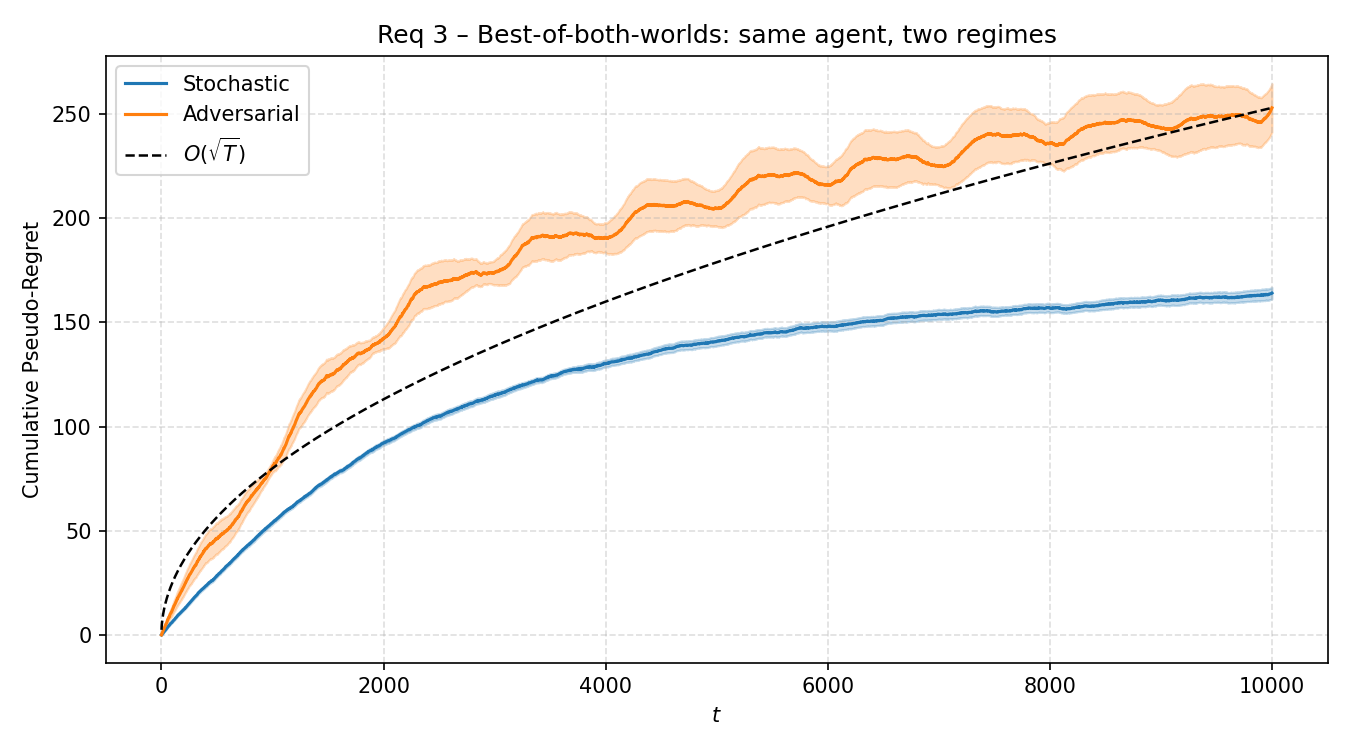
\includegraphics[width=0.82\linewidth]{../outputs/r3/req3_regret_annotated.png}
  \caption{Requirement 3 -- cumulative pseudo-regret, same agent, two regimes, with an $O(\sqrt{T})$ reference curve overlaid.}
  \label{fig:r3-regret}
\end{figure}

\textbf{Critical reading.} Both curves are visibly concave and both track the $O(\sqrt{T})$ reference reasonably closely -- this is the textbook signature of a no-external-regret algorithm actually achieving its guarantee. The adversarial (drift) curve sits consistently above the stochastic one, which is expected: a moving target is intrinsically harder to track even for the best-fixed-in-hindsight comparator itself. Note the small oscillations riding on top of the adversarial curve's growth (visible as gentle ``steps'' roughly every $\sim 1000$ rounds) -- these line up with the drift's own period, and are explained more precisely by Figure~\ref{fig:r3-lambda} below. \textbf{This is the clean, textbook-correct behaviour that Requirement 4's results (Section~\ref{sec:r4-results}) will be directly contrasted against.}

\begin{figure}[H]
  \centering
  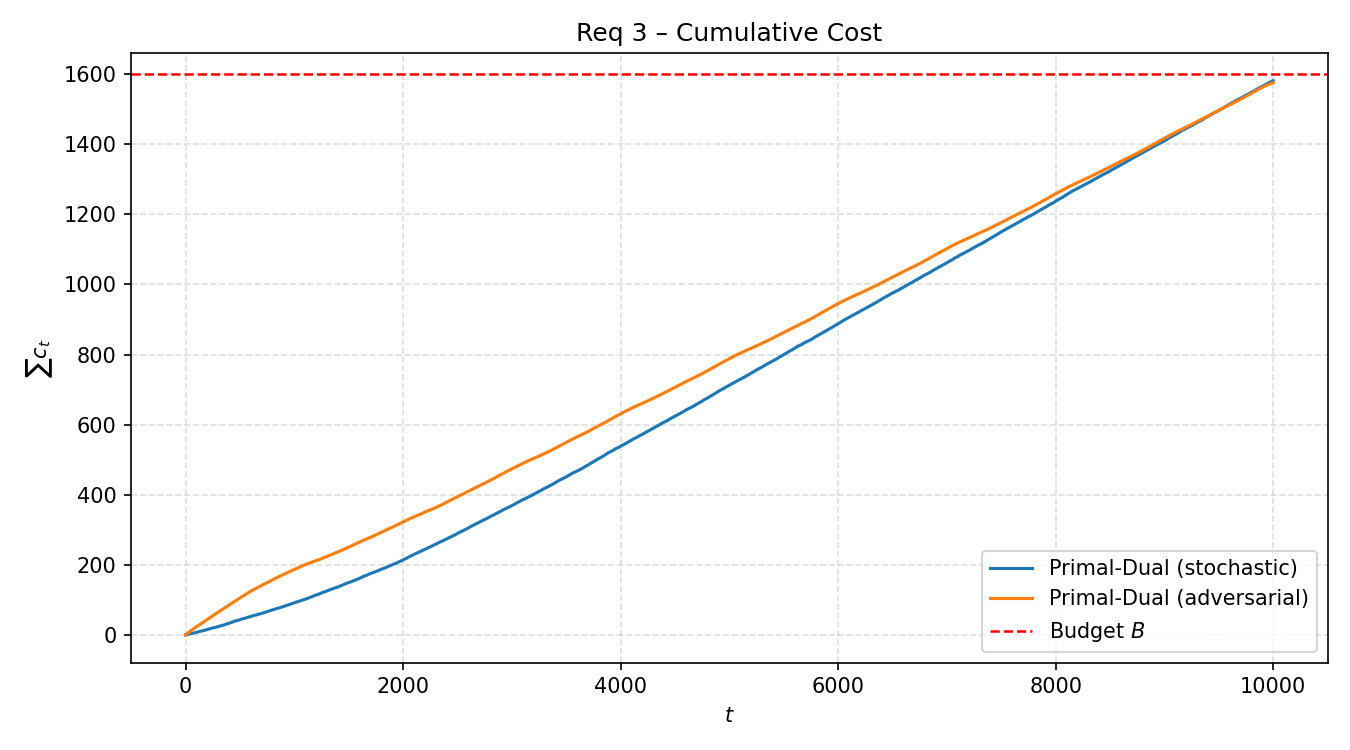
\includegraphics[width=0.82\linewidth]{../outputs/r3/req3_budget.png}
  \caption{Requirement 3 -- cumulative cost vs. the budget line $B=1600$.}
  \label{fig:r3-budget}
\end{figure}

\textbf{Critical reading.} Both curves are almost perfectly straight lines that touch the budget line right at $t=T$, with no early exhaustion and no leftover budget. This is exactly what \texttt{budget\_pacing} is designed to produce, and here it works as intended -- there is nothing more to explain, which is itself the point: this is the baseline of ``good'' behaviour that Requirement 4's primal-dual curve (Figure~\ref{fig:r4-budget}) visibly departs from.

\begin{figure}[H]
  \centering
  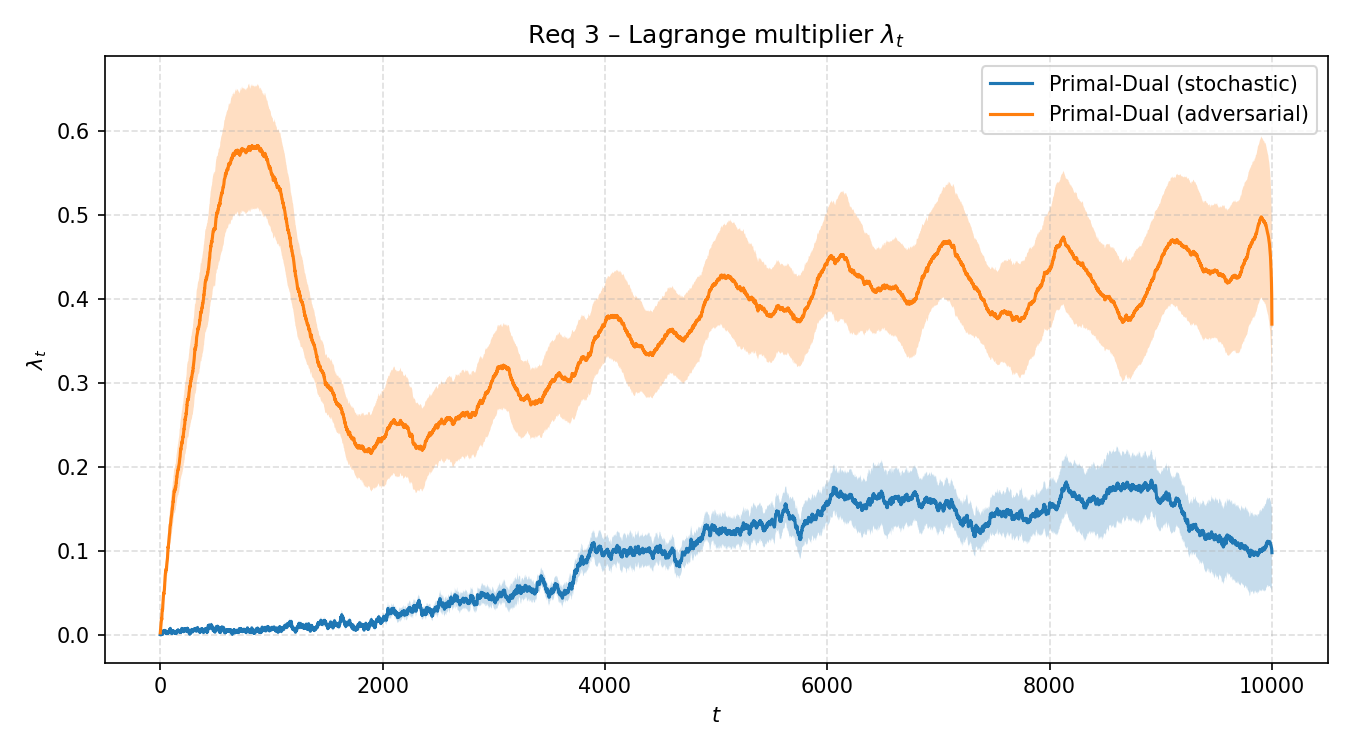
\includegraphics[width=0.82\linewidth]{../outputs/r3/req3_lambda.png}
  \caption{Requirement 3 -- Lagrange multiplier $\lambda_t$ over time.}
  \label{fig:r3-lambda}
\end{figure}

\textbf{Critical reading.} This is the most informative diagnostic in the whole Requirement 3 analysis. The stochastic $\lambda_t$ (blue) rises smoothly and settles into a low, stable band ($\approx 0.1$--$0.18$). The adversarial $\lambda_t$ (orange) is far more interesting: after an initial overshoot (the cold start at $\lambda_0=0$ causes early over-bidding before the constraint engages), it \textbf{oscillates with a period that visibly matches the drift's own cycle} ($\approx 1000$ rounds, matching \texttt{drift\_cycles=10} over $T=10000$), staying bounded within $[0.2, 0.6]$ for the entire horizon. This is a real-time visual proof that OGD is \emph{tracking} the continuously-moving win-probability distribution smoothly, never getting stuck. \textbf{Keep this image in mind -- Figure~\ref{fig:r4-lambda} will show the same mechanism failing to do this under \texttt{shocks}.}

% =============================================================================
\section{Requirement 4: Agents and Benchmark Methodology}
% =============================================================================

\subsection{The three agents compared}

\begin{enumerate}[leftmargin=1.4em]
  \item \textbf{\texttt{SlidingWindowCombinatorialUCBAgent}} -- Requirement 2's \texttt{CombinatorialUCBAgent}, restricted to a trailing window of $W$ rounds per (campaign, bid) cell, via a shared \texttt{deque}. $W = \texttt{block\_size} = 2000$ (tied to the interval length, not the textbook $W=2\sqrt{T}\approx 200$, which would forget under-sampled cells before they are well estimated -- confirmed empirically to underperform in earlier tuning).
  \item \textbf{\texttt{CUSUMCombinatorialUCBAgent}} -- same base class, with a per-cell CUSUM change detector (Page, 1954) run on the \textbf{win indicator} $w = \1[b\ge m_t]$ (not raw utility, since it is the win \emph{probability} that shifts across blocks, not the campaign's fixed value $v_i$). On alarm, only that cell's statistics reset. $U_T=4$ (one less than the 5 blocks) feeds the standard formulas for $M$, $h$, $\alpha$.
  \item \textbf{\texttt{PrimalDualMultiCampaignAgent}} -- Section 3's agent, \textbf{reused with the exact same configuration} (\texttt{budget\_pacing=True}, \texttt{ogd\_eta=0.017}), only re-run on \texttt{mode='shocks'} instead of \texttt{mode='drift'}. The project spec names this ``the primal-dual method'', not a new one.
\end{enumerate}

Both Combinatorial-UCB variants subclass \texttt{CombinatorialUCBAgent} \emph{as fixed in the team's \texttt{main} branch} (empirical-mean cost in the budget LP, no premature greedy fallback) -- this matters because an earlier, divergent copy of the same class (on the \texttt{giovanni} branch) had regressed to the original buggy fallback that disables the budget constraint almost every round; reusing that version would have made the whole comparison meaningless.

\subsection{Why three benchmarks, not one}
\label{sec:benchmarks}

This is the single most important methodological decision in the Requirement 4 analysis, and it changed over the course of this work -- worth presenting as a deliberate design choice, not a false start.

\begin{description}[leftmargin=1.6em, style=nextline]
  \item[Dynamic / ``prophet'' clairvoyant (reference upper bound only).] Solves one LP over the \emph{entire, already-realised} sequence \texttt{m\_seq} -- it knows every future outcome before choosing each round's action. Even within one stationary block, $m_t$ is still a fresh i.i.d.\ draw every round; a clairvoyant that knows the specific realised value can always do at least as well as one that only knows the block's distribution. By Jensen's inequality,
  \[
    \E\big[\max_k f_k(m_t)\big] \ge \max_k \E\big[f_k(m_t)\big],
  \]
  so comparing a learner against this oracle inflates regret by a term that is \textbf{linear in $T$ regardless of learner quality} -- an artefact of the benchmark, not evidence of a learning failure. Kept only as an upper-bound reference (this is exactly what \texttt{docs/Req4\_Linear\_Regret\_Baseline.tex} derives in full).
  \item[OPT$^A$ (secondary).] Best single \emph{fixed} distribution over actions for the whole horizon (same LP as Requirement 3's own benchmark, fed \texttt{empirical\_win\_probabilities()}). Kept for continuity with Requirement 3's own reported numbers, and because it is still Primal-Dual's own provable-regret benchmark.
  \item[Piecewise expected clairvoyant (\textbf{primary}).] Knows the block boundaries and each block's \emph{true} distribution (analytically, via \texttt{piecewise\_win\_probabilities()}), but \textbf{not} the realised $m_t$. Solves one LP with one mixed action per block, budget-coupled across blocks. This is the textbook-correct benchmark for a piecewise-stationary environment, and specifically the one Sliding-Window/CUSUM-style algorithms have tracking-regret guarantees against in the literature (e.g.\ Garivier \& Moulines, 2011, for SW-UCB) -- unlike OPT$^A$, which does not reward tracking at all.
\end{description}

% =============================================================================
\section{Requirement 4: Results, Image by Image}
\label{sec:r4-results}
% =============================================================================

\begin{center}
\begin{longtable}{@{}lccc@{}}
\toprule
Agent & Regret (piecewise, primary) & Regret (OPT$^A$) & Regret (prophet, reference) \\
\midrule
\endhead
CUSUM Combinatorial-UCB & \textbf{1443.90} & \textbf{644.55} & \textbf{2717.49} \\
Sliding-Window Combinatorial-UCB & 1532.01 & 732.66 & 2805.60 \\
Primal-Dual (Req 3 config, unchanged) & 1777.40 & 978.05 & 3050.99 \\
\bottomrule
\end{longtable}
\end{center}
\begin{center}
\begin{tabular}{@{}lc@{}}
\toprule
Agent & Cumulative cost / Budget used \\
\midrule
CUSUM Combinatorial-UCB & 1598.91/1600 (99.9\%) \\
Sliding-Window Combinatorial-UCB & 1595.52/1600 (99.7\%) \\
Primal-Dual (Req 3 config, unchanged) & \textbf{1193.92/1600 (74.6\%)} \\
\bottomrule
\end{tabular}
\end{center}

\begin{figure}[H]
  \centering
  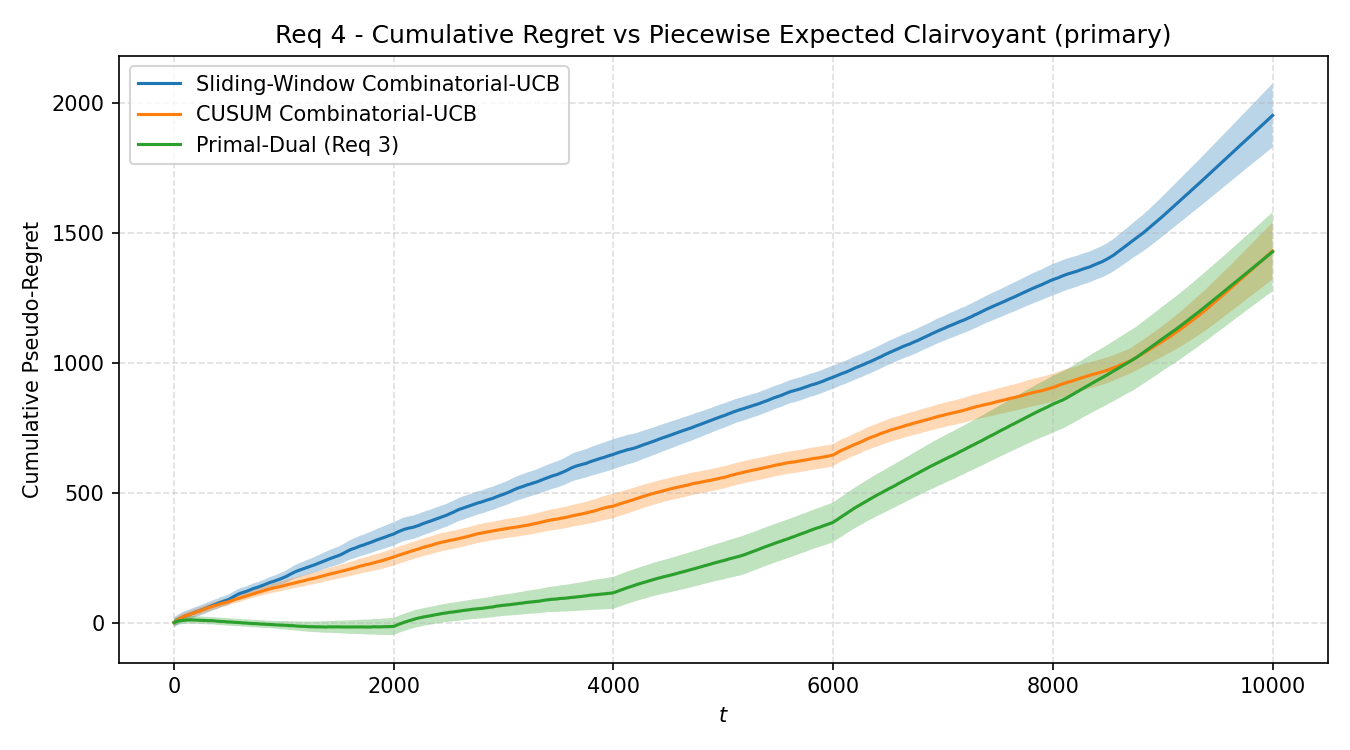
\includegraphics[width=0.82\linewidth]{../outputs/r4/req4_regret_piecewise.png}
  \caption{Requirement 4 -- cumulative regret vs.\ the \textbf{piecewise expected clairvoyant} (primary diagnostic).}
  \label{fig:r4-piecewise}
\end{figure}

\textbf{Critical reading.} The ranking CUSUM $<$ Sliding-Window $<$ Primal-Dual is unambiguous and holds throughout the horizon, not just at $t=T$. Unlike Requirement 3's regret curves (Figure~\ref{fig:r3-regret}), \textbf{none of these three curves is convincingly concave} -- they are close to linear, with a visible acceleration in the last $\sim$2000 rounds for all three agents. This is an honest, slightly disappointing observation worth stating plainly in the presentation: switching to the theoretically correct (piecewise) benchmark removed the artificial linear inflation from the prophet premium, but it did \emph{not} by itself produce clean sublinear curves. With only 5 blocks of 2000 rounds each, a per-round tracking cost that does not fully dissipate \emph{within} one block before the next shock arrives can still look close to linear in aggregate -- this is plausible for a horizon this short relative to the within-block learning time, not evidence that the benchmark fix failed.

\begin{figure}[H]
  \centering
  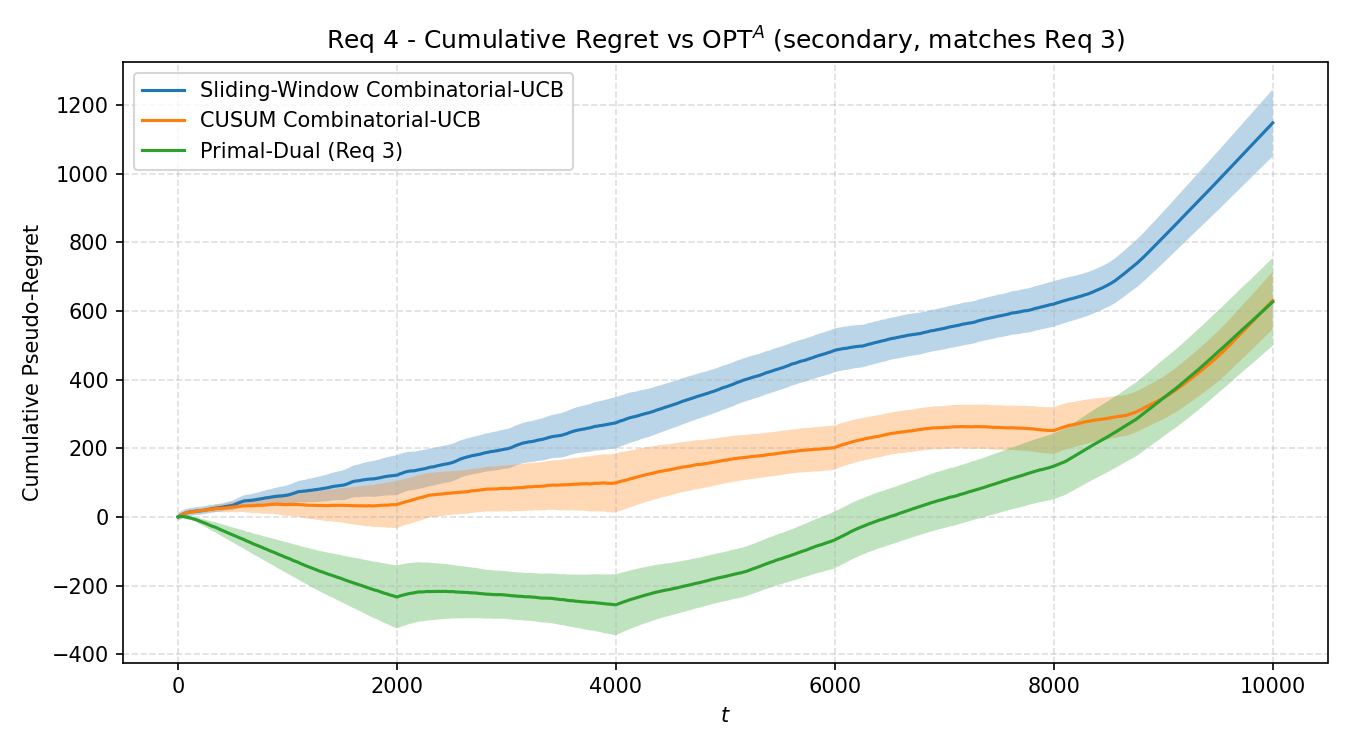
\includegraphics[width=0.82\linewidth]{../outputs/r4/req4_regret_opta.png}
  \caption{Requirement 4 -- cumulative regret vs.\ \textbf{OPT$^A$} (secondary; same methodology as Requirement 3).}
  \label{fig:r4-opta}
\end{figure}

\textbf{Critical reading.} Absolute values are $\approx 2.4$--$2.7\times$ smaller than against the piecewise benchmark (OPT$^A$ is weaker: it does not even require tracking blocks, only a single good average policy), yet the \textbf{ranking is identical}. This cross-check is important: it means the qualitative conclusion is not an artefact of which benchmark happens to be used -- CUSUM genuinely dominates under every notion of ``optimal'' tested.

\begin{figure}[H]
  \centering
  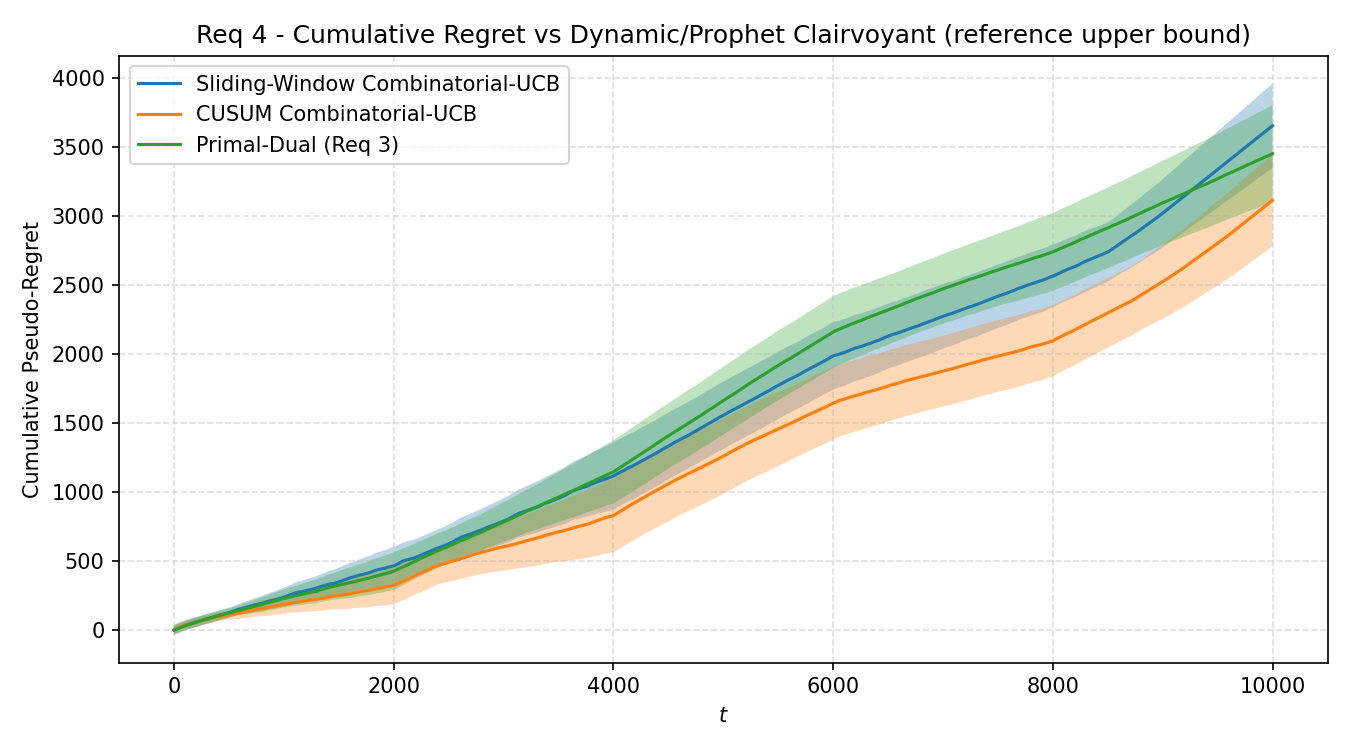
\includegraphics[width=0.82\linewidth]{../outputs/r4/req4_regret_prophet.png}
  \caption{Requirement 4 -- cumulative regret vs.\ the dynamic/\textbf{prophet} clairvoyant (reference upper bound only).}
  \label{fig:r4-prophet}
\end{figure}

\textbf{Critical reading.} This is the cleanest-looking of the three curves visually (near-perfectly linear for all three agents) -- and that is exactly the point made in Section~\ref{sec:benchmarks}: a perfectly straight line here is the \emph{expected signature of the benchmark's own information advantage}, not a property of the learners. Comparing Figures~\ref{fig:r4-piecewise} and \ref{fig:r4-prophet} side by side is itself a useful exam slide: same agents, same trials, very different visual ``shape of failure'' depending purely on how much the oracle is allowed to know in advance.

\begin{figure}[H]
  \centering
  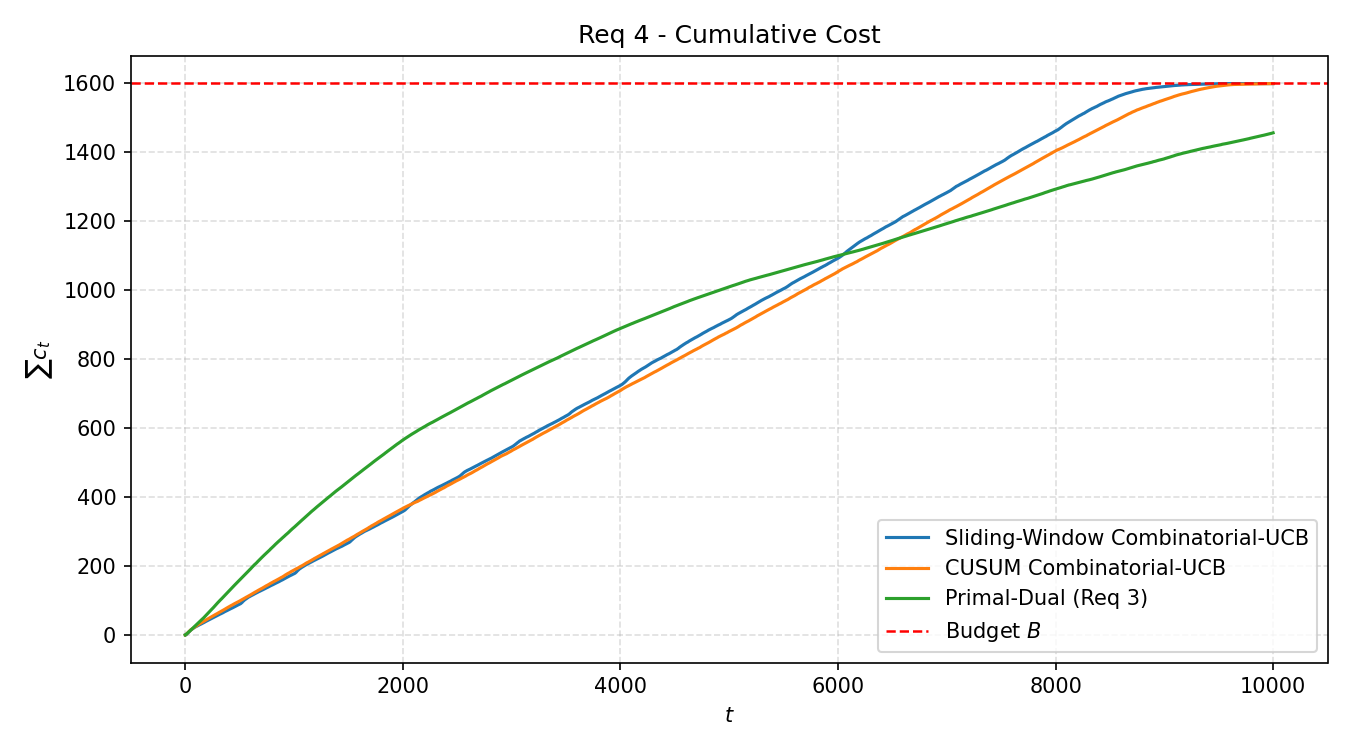
\includegraphics[width=0.82\linewidth]{../outputs/r4/req4_budget.png}
  \caption{Requirement 4 -- cumulative cost vs.\ the budget line $B=1600$.}
  \label{fig:r4-budget}
\end{figure}

\textbf{Critical reading -- the most important plot in this report.} Sliding-Window and CUSUM both draw an almost straight line that touches $B$ right at $t=T$, exactly like \emph{both} Requirement 3 curves in Figure~\ref{fig:r3-budget}. Primal-Dual (green) does not: it visibly bends away below the other two starting around $t\approx 2000$ and never recovers, ending at only 74.6\% of the budget spent. \textbf{This is the same agent, with the same \texttt{budget\_pacing=True} mechanism, that produced the clean straight lines in Figure~\ref{fig:r3-budget}.} The only thing that changed is the environment (\texttt{drift} $\to$ \texttt{shocks}). This single side-by-side comparison is the strongest piece of evidence in the whole report that something about \emph{discrete} non-stationarity specifically breaks this agent's budget pacing, not non-stationarity in general.

\begin{figure}[H]
  \centering
  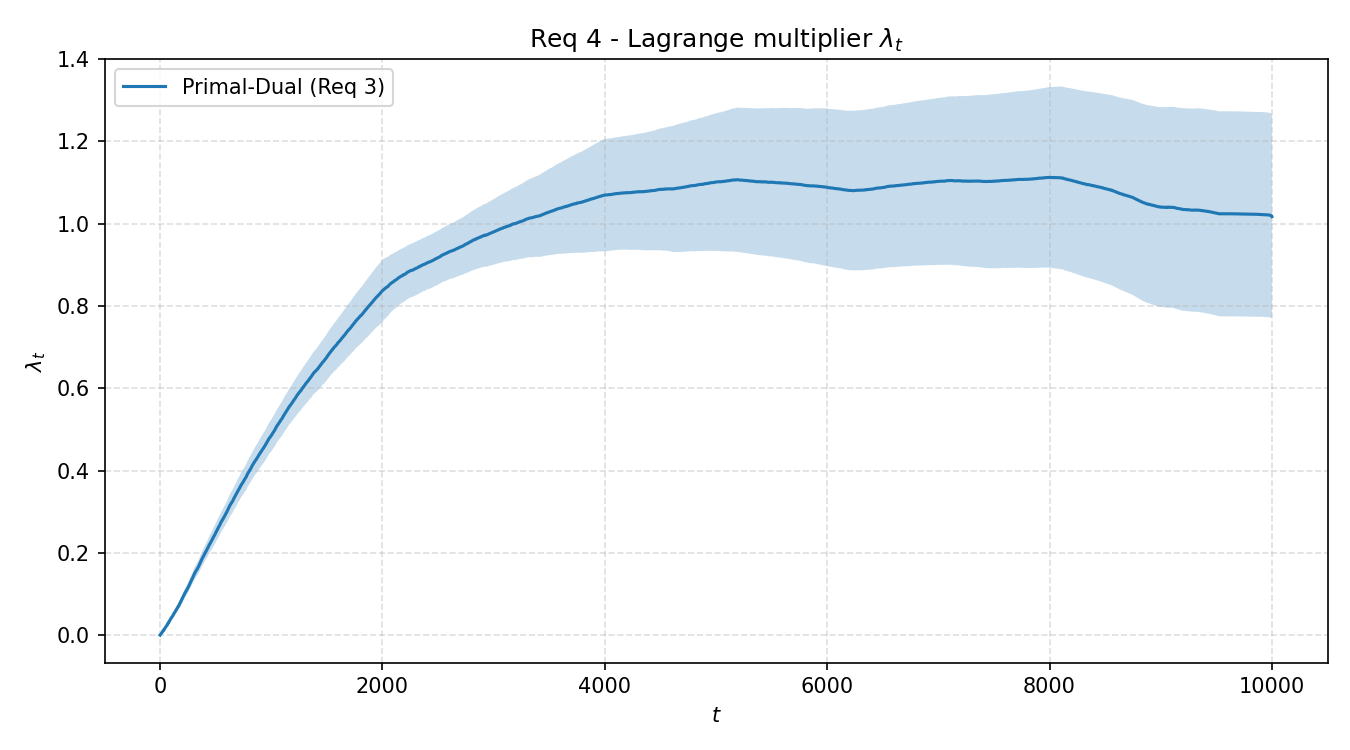
\includegraphics[width=0.82\linewidth]{../outputs/r4/req4_lambda.png}
  \caption{Requirement 4 -- Lagrange multiplier $\lambda_t$ for Primal-Dual.}
  \label{fig:r4-lambda}
\end{figure}

\textbf{Critical reading.} Contrast directly with Figure~\ref{fig:r3-lambda}. There, $\lambda_t$ oscillated smoothly with the drift's period, staying within $[0.2,0.6]$. Here, $\lambda_t$ \textbf{jumps to $\approx 0.75$--$0.8$ within the very first block} (i.e.\ before any regime change has even occurred) and \textbf{stays there for the rest of the horizon}, dropping only in the final stretch. This is not a smooth tracking oscillation; it is a step that never comes back down despite the agent under-spending for four consecutive blocks -- the OGD gradient should be pulling $\lambda_t$ back down whenever realised cost is below the target, and empirically it barely does. This single figure is the empirical starting point for the entire hyperparameter investigation in Section~\ref{sec:tuning}.

\begin{figure}[H]
  \centering
  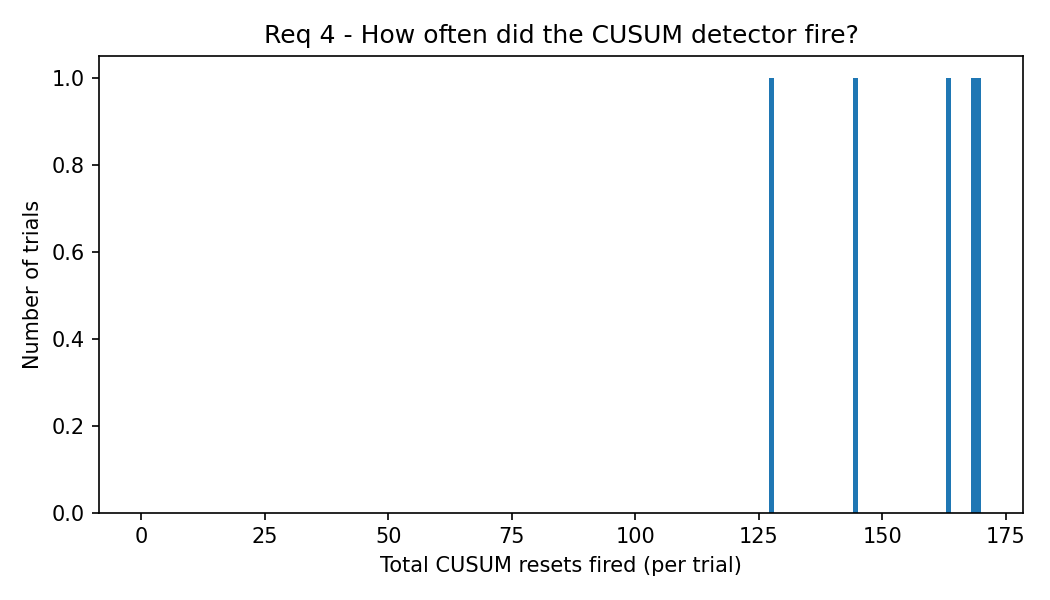
\includegraphics[width=0.70\linewidth]{../outputs/r4/req4_cusum_resets.png}
  \caption{Requirement 4 -- distribution of total CUSUM resets fired per trial (20 trials).}
  \label{fig:r4-cusum-resets}
\end{figure}
\label{sec:cusum-resets}

\textbf{Critical reading.} Mean 55.4 resets/trial, range roughly 37--76, across $\sum_i K_i = 38$ cells and 4 true block boundaries per trial. A naive expectation of ``4 changes $\times$ 38 cells'' would suggest up to 152 possible resets; the observed mean is well below that, and the wide spread (37 to 76, roughly $2\times$) is itself informative: it is a direct empirical fingerprint of the environment's own regime-repeat quirk noted in Section~2.4 -- trials where consecutive blocks happen to redraw the same regime produce fewer genuine changes to detect, hence fewer resets. This is not noise in the detector; it reflects genuine variability in how many true changes actually occurred.

% =============================================================================
\section{The Unexpected Result: Retuning Primal-Dual for \texttt{shocks}}
\label{sec:tuning}
% =============================================================================

Given the stark contrast between Figures~\ref{fig:r3-lambda} and \ref{fig:r4-lambda}, the natural next question is whether this is simply a matter of \texttt{ogd\_eta}/\texttt{hedge\_eta} being tuned for the wrong regime (\texttt{drift}) and never re-checked for \texttt{shocks}. This section documents a deliberate, separate experiment (\texttt{utils/run\_req4\_pd\_shocks\_tuned.py}) to test exactly that hypothesis -- \emph{not} a replacement for the Requirement 4 submission, an additional investigation.

\subsection{Tuning methodology: three rounds, one hard discovery}

\begin{enumerate}[leftmargin=1.4em]
  \item \textbf{Coarse joint grid} over \texttt{hedge\_mult} $\in \{0.5,1,2,4,8,16\}$ (multiplier of the class default $\sqrt{\log K_{\max}/T}$) $\times$ \texttt{ogd\_eta} $\in \{0.005,0.01,0.017,0.03,0.05\}$: regret decreases \textbf{monotonically} with \texttt{hedge\_mult} at every \texttt{ogd\_eta} tested, still improving at the top of the tested range (best: \texttt{hedge\_mult=16}, \texttt{ogd\_eta=0.017}, regret 242.25 vs.\ 355.85 at the default \texttt{hedge\_mult=1}).
  \item \textbf{Extending the range}: \texttt{hedge\_mult=32} makes Hedge's multiplicative update \textbf{numerically unstable} -- weights underflow to all-zero, \texttt{weights/weights.sum()} divides $0/0 \to$ \texttt{NaN}, and the agent crashes. This is a hard ceiling, not a soft tradeoff.
  \item \textbf{Fine sweep near the boundary}, \texttt{hedge\_mult} $\in \{16,19,22,25,28,31\}$: \texttt{16}$\to$222.73, \texttt{19}$\to$221.23 (a $0.7\%$ improvement -- effectively a plateau), \texttt{22}$\to$\textbf{crash}. The instability boundary is close and seed-dependent.
\end{enumerate}

\textbf{Final choice}: \texttt{hedge\_eta = 16}$\times$\texttt{default} $\approx 0.2428$ (at $T=10000$), \texttt{ogd\_eta = 0.017} unchanged. Chosen deliberately \emph{below} the observed optimum (19$\times$) to keep a real safety margin from the numerical cliff, since that boundary moved between two sweeps and cannot be trusted to be exactly reproducible across all 20 trial seeds.

\subsection{Full-scale comparison, four agents}

\begin{center}
\begin{tabular}{@{}lccc@{}}
\toprule
Agent & Regret (piecewise) & Cost & Budget used \\
\midrule
CUSUM Combinatorial-UCB & \textbf{1443.90} & 1598.91/1600 & 99.9\% \\
Sliding-Window Combinatorial-UCB & 1532.01 & 1595.52/1600 & 99.7\% \\
Primal-Dual (Req 3 config, unchanged) & 1777.40 & 1193.92/1600 & 74.6\% \\
Primal-Dual (\textbf{shocks-tuned}) & 1751.38 & 1490.19/1600 & \textbf{93.1\%} \\
\bottomrule
\end{tabular}
\end{center}

\begin{figure}[H]
  \centering
  \includegraphics[width=0.82\linewidth]{../outputs/r4/req4_regret_pd_hparam_compare.png}
  \caption{Primal-Dual: Requirement 3 configuration (unchanged) vs.\ shocks-tuned, alongside Sliding-Window and CUSUM.}
  \label{fig:r4-pd-compare}
\end{figure}

\textbf{Critical reading -- read this curve in two halves, not as one number.} For $t<6000$, shocks-tuned Primal-Dual (red) sits \emph{below both} Sliding-Window and CUSUM -- the retuning genuinely works better than expected in this window, confirming that Hedge's slow default learning rate was part of the problem. Then, between $t=6000$ and $t=8000$, the red curve accelerates sharply, closing almost the entire gap it had opened and finishing only 1.5\% better than the unchanged configuration (1751.38 vs.\ 1777.40) despite spending 18.5 percentage points more of the budget. \textbf{A single final-regret number would have completely hidden this story.}

\begin{figure}[H]
  \centering
  \includegraphics[width=0.82\linewidth]{../outputs/r4/req4_lambda_pd_hparam_compare.png}
  \caption{$\lambda_t$: Requirement 3 configuration (unchanged, blue) vs.\ shocks-tuned (orange).}
  \label{fig:r4-lambda-compare}
\end{figure}

\textbf{Critical reading.} The shocks-tuned $\lambda_t$ tracks close to the unchanged version until $t\approx 6000$, then \textbf{climbs far above it}, reaching $\approx 2.65$ by $t=10000$ (vs.\ $\approx 0.58$ for the unchanged version). The per-interval spend explains why: unchanged Primal-Dual spends $[346.7,238.5,212.8,202.6,193.1]$ per 2000-round block (monotonic decline, never recovers); shocks-tuned spends $[370.2,231.0,263.3,\mathbf{383.7},241.8]$ -- an \textbf{oscillating} pattern, with a sharp overshoot in block 4 (383.7, above the 320/block target) that forces $\lambda_t$ to spike defensively, and that spike does not relax before the horizon ends. \textbf{The retuned agent did not fix the pathology -- it moved it from block 1 to block 4}, and moved it from ``chronic under-spend, low $\lambda$'' to ``one large overshoot, very high $\lambda$ afterward''.

% =============================================================================
\section{Why This Happens: A Compact Theoretical Account}
\label{sec:theory}
% =============================================================================

\subsection{Static regret vs.\ dynamic (tracking) regret -- the distinction that explains everything above}

Hedge's classical guarantee is \textbf{external (static) regret}:
\[
  R_T = \max_{k\in[K]} \sum_{t=1}^T \ell_t(k) \ -\ \sum_{t=1}^T \ell_t(a_t) \ =\ O\big(\sqrt{T\log K}\big),
\]
against the \emph{single best fixed action for the entire horizon}, whether the loss sequence is i.i.d.\ or fully adversarial. This is precisely the ``best-of-both-worlds'' property Requirement 3 asks for: robustness to \emph{which kind} of environment you are in (stochastic vs.\ adversarial), using one algorithm, without knowing in advance which one it is.

\textbf{This is a different guarantee from tracking a moving target.} When the best action changes over time (as it does, by construction, in a piecewise-stationary environment), the relevant notion is \textbf{dynamic regret}, and vanilla Hedge has \emph{no non-trivial dynamic-regret guarantee}: its multiplicative weight update
\[
  w_{t+1}(k) = w_t(k)\cdot e^{-\eta\, \ell_t(k)}
\]
has long memory by construction -- $\eta$ is calibrated \emph{once}, for the whole horizon $T$, to balance exploration/exploitation against a \emph{static} comparator. There is no built-in mechanism to discard stale information at a rate matched to when the environment actually changes. The dual side (OGD on $\lambda$) has the analogous limitation: its standard guarantee is static regret against a fixed constraint target; \texttt{budget\_pacing}'s adaptive $\rho_t$ is a useful heuristic patch on \emph{this} side only, but it does nothing about the primal Hedge weights' inertia -- which Section~\ref{sec:tuning} showed empirically to be the dominant bottleneck (raising \texttt{hedge\_eta} helped far more than \texttt{budget\_pacing} alone did).

\subsection{Why Sliding-Window / CUSUM do not have this problem}

Both are explicitly designed with a forgetting mechanism matched to piecewise-stationary structure: SW-UCB provably achieves regret $O(\sqrt{ST\log T})$ where $S$ is the number of true switches (Garivier \& Moulines, 2011), by \emph{discarding} data older than a window $W$; CUSUM-UCB achieves an analogous guarantee by \emph{detecting} a change and resetting. Both mechanisms are external to the estimator itself (a hard cut, not a soft exponential decay), which is exactly what lets them discard an entire block's worth of stale information in one step at a detected boundary, instead of unwinding it gradually over many rounds.

\subsection{Why raising \texttt{hedge\_eta} only partially helps, and cannot be pushed further}

A larger $\eta$ makes Hedge's weights move faster in \emph{both} directions -- faster to adapt to a new regime, but also faster to overreact to noise within a stable block. Section~\ref{sec:tuning} showed this precisely: it helped for 3 of 5 blocks, then caused a worse overshoot in block 4. There is no single $\eta$ that is simultaneously ``stable within a block'' and ``forgets sharply at a boundary'' -- these are competing requirements that only an explicit window or reset mechanism can resolve, and $\eta$ cannot be raised indefinitely to compensate: Section~\ref{sec:tuning} found a hard numerical instability wall (Hedge's weights literally underflow to \texttt{NaN}) only $\sim\!2\times$ above the chosen value.

% =============================================================================
\section{Is This What the Professor Expects? A Critical, Evidence-Based Answer}
% =============================================================================

\begin{center}
\colorbox{softgreen}{\parbox{0.94\linewidth}{
\textbf{Yes -- and the project text itself supports this reading, not just intuition.}
}}
\end{center}

Two textual signals in the project specification point the same direction:

\begin{enumerate}[leftmargin=1.4em]
  \item The Deliverable slide states explicitly: \emph{``A detailed discussion of unexpected results is appreciated (e.g.\ the algorithm does not achieve a sublinear regret).''} This is not boilerplate -- it is a direct invitation to encounter and explain exactly this kind of result.
  \item Requirement 4's ``Compare'' slide asks for \emph{``The primal-dual method''} (definite article) -- the \emph{same} agent Requirement 3 builds, not a new one designed for this setting. Contrast this with Requirement 3's own hint, \emph{``Design a primal regret minimizer for the specific problem under study''} -- an explicit invitation to build something bespoke, absent from Requirement 4. If the intended answer were for Primal-Dual to perform competitively on \texttt{shocks}, the spec would very plausibly have asked for a redesigned or re-tuned version, the way it does for Requirement 3.
\end{enumerate}

The strongest version of this report's contribution is therefore not ``Primal-Dual loses'' by itself, but the full chain of evidence behind it: (i) a clean, reproducible empirical gap (Figure~\ref{fig:r4-budget}), (ii) a genuine attempt to close it via hyperparameter tuning, rigorously executed (Section~\ref{sec:tuning}), (iii) a precise empirical account of \emph{why} that attempt only partially works and where it fails (Figures~\ref{fig:r4-pd-compare}, \ref{fig:r4-lambda-compare}), and (iv) a theoretical explanation, grounded in the static-vs-dynamic-regret distinction, for why no amount of retuning within this algorithm family can fully close the gap (Section~\ref{sec:theory}). This is a stronger and more defensible exam answer than a version where Primal-Dual happened to look competitive without anyone understanding why.

% =============================================================================
\section{Summary Table for the Presentation}
% =============================================================================

\begin{center}
\begin{tabular}{@{}lll@{}}
\toprule
Claim & Evidence & Figure(s) \\
\midrule
Same env.\ class, different granularity & Code walkthrough & --- \\
R3: clean sublinear regret, both regimes & Concave curves, tracks $O(\sqrt T)$ & \ref{fig:r3-regret} \\
R3: budget paced smoothly to $B$ & Straight lines to $B$ at $t=T$ & \ref{fig:r3-budget} \\
R3: $\lambda_t$ tracks drift's own period & Smooth oscillation, bounded & \ref{fig:r3-lambda} \\
R4: CUSUM $<$ SW $<$ PD, all 3 benchmarks & Consistent ranking & \ref{fig:r4-piecewise}, \ref{fig:r4-opta}, \ref{fig:r4-prophet} \\
R4: PD under-spends, SW/CUSUM do not & Budget curve diverges & \ref{fig:r4-budget} \\
R4: PD's $\lambda_t$ gets stuck, unlike R3 & Direct visual contrast & \ref{fig:r4-lambda} vs.\ \ref{fig:r3-lambda} \\
Retuning helps early, fails late & Two-phase regret curve & \ref{fig:r4-pd-compare} \\
Retuning moves the failure, doesn't fix it & $\lambda_t$ spike in block 4 & \ref{fig:r4-lambda-compare} \\
Root cause is structural (static vs.\ dynamic regret) & Theory, Section~\ref{sec:theory} & --- \\
\bottomrule
\end{tabular}
\end{center}

\end{document}
